\documentclass[conference]{IEEEtran}
\usepackage{amsmath,amssymb}
\usepackage{graphicx}
\usepackage{booktabs}
\usepackage[section]{placeins}
\usepackage{stfloats}
\usepackage{array}
\usepackage[hidelinks]{hyperref}
\graphicspath{{figures/}}
\renewcommand{\arraystretch}{1.12}
\renewcommand{\topfraction}{0.9}
\renewcommand{\dbltopfraction}{0.9}
\renewcommand{\textfraction}{0.07}
\renewcommand{\floatpagefraction}{0.85}
\renewcommand{\dblfloatpagefraction}{0.85}
\setcounter{topnumber}{3}
\setcounter{dbltopnumber}{2}

\begin{document}

\title{Statistical Modelling of Packet-Loss Patterns in Computer Networks: Distribution Fitting, Burstiness Testing and Bayesian Estimation}

\author{\IEEEauthorblockN{BAMAT207 Probability and Statistics: Case Study Report}}

\maketitle

\begin{abstract}
A network's loss rate is usually quoted as a single number, and most simple models treat each lost packet as an independent event. If that were true, losses per second would follow a Poisson distribution and the gaps between losses would be exponential. We wanted to see how well this holds up when losses come in bursts. We simulated three kinds of network (wired broadband, campus Wi-Fi and a mobile hotspot) with a two-state Gilbert-Elliott model, sending 50 packets per second for 1 hour on each, so 180{,}000 packets per network. We then fitted count and waiting-time models, tested whether consecutive packets are independent, and estimated loss rates with a Bayesian Beta-Binomial model. The independence assumption failed on every network. The variance of losses per second was 1.59, 5.31, 10.17 times the mean, where Poisson predicts 1, and a single loss made the next one 31 to 43 times more likely. This matters in practice: across 2{,}000 simulated captures, the usual 95\% interval for the loss rate caught the true value only 40.3\% to 85.7\% of the time. Shrinking the sample size by a design effect brought coverage back to 93.3\% to 94.0\%. A power study tells us to record at least ten minutes per network when we move on to real measurements.
\end{abstract}

\begin{IEEEkeywords}
packet loss, Gilbert-Elliott model, burstiness, goodness of fit, Bayesian estimation, design effect, Monte Carlo simulation
\end{IEEEkeywords}

\section{Introduction}
Anyone who has been on a video call over a weak Wi-Fi connection knows what packet loss feels like. The picture freezes for a moment, the voice drops a word, and then everything carries on. Behind this, the call is sending small packets at a steady rate, and some of them never arrive. The share that goes missing is the loss rate. It is the number that appears in service agreements, and it is what protocol designers use when they set retransmission timers or decide how much error correction to add.

The trouble is that the loss rate only tells you how many packets were lost, not when. Ten lost packets spread over a minute are barely noticeable, because the decoder can patch over a single gap. Ten lost packets in a row are a visible freeze. Most textbook treatments get around this by assuming that every packet is lost independently, with the same small probability $p$. That assumption is convenient. It makes the number of losses in a short window Binomial, which is very close to Poisson, and it makes the time between losses exponential. If losses actually cluster together, both of these results stop being true, and so do the error bars that are built on them.

We set out to measure how badly the independence assumption breaks, which standard tests can detect it, and what it does to the interval estimates people report for the loss rate. The project has two phases. This report covers Phase 1, a simulation study. Because we chose the true parameters of each network ourselves, we can check every estimate and every test against the right answer before trusting the same code on real data. Phase 2 will run that code on real captures.

Concretely, we fit two models to the per-second loss counts (Poisson and Negative Binomial) and two to the gaps between losses (exponential and a two-phase mixture). We test independence with a runs test and a Markov-chain likelihood-ratio test, and we estimate burst behaviour with a Bayesian model. Finally, we use simulation to check how often the usual 95\% interval actually works, and how long a real capture needs to be.

The rest of the report runs as follows. Section~II gives the background, Section~III describes the loss model and how the data were generated, Section~IV explains the statistical methods, and Section~V presents the results. Section~VI discusses what the results mean and where the study falls short, and Section~VII sums up.

\section{Background}
The idea of modelling bursty errors with a hidden two-state chain goes back to E.~N.~Gilbert's work on telephone lines in 1960. E.~O.~Elliott extended it in 1963 so that errors could happen in both states, and the Gilbert-Elliott model is still the usual first choice for describing bursty loss.

It has also been known for a long time that Internet losses are not independent. Measurement studies in the 1990s found that probe packets sent close together tend to be lost together, that loss in TCP transfers comes in correlated episodes, and that Markov chains describe the time pattern of loss in multicast traces quite well. Later work fitted Gilbert models to voice traffic and linked the length of a burst to how bad a call sounds.

Most of that work is about describing the loss process itself. Our angle is more statistical. We want to know which standard tests pick up the dependence, how much data they need to do it, and how far ordinary interval estimates drift when the dependence is ignored. For the last question we borrow the idea of a design effect from survey sampling, where it is used to correct for people being sampled in clusters rather than one at a time.

\section{Loss Model and Data}
\subsection{The Gilbert-Elliott Channel}
Think of the network as having two moods, Good (G) and Bad (B). We cannot see the mood directly, only its effect. Before each packet, the channel moves from Good to Bad with probability $p$, and from Bad back to Good with probability $r$. A packet is lost with a small probability $h_G$ in the Good state and a much larger probability $h_B$ in the Bad state. In the long run, the flow into Bad has to match the flow out of it, which gives the share of time spent in Bad and the overall loss rate:
\begin{equation}
\pi_B=\frac{p}{p+r},\qquad P(\text{loss})=(1-\pi_B)\,h_G+\pi_B\,h_B .
\label{eq:ge}
\end{equation}
Each stay in a state lasts a geometric number of packets. The average stay is $1/p$ packets in Good and $1/r$ in Bad. A burst of losses happens when the channel slips into Bad for a few packets.

\subsection{Scenarios and Sampling}
Table~\ref{tab:params} lists the parameters for our three networks. We picked them to give a low, a medium and a high loss rate, with the Bad spells getting longer as the network gets worse. Each network sends a steady 50 packets per second, one every 20~ms, which is roughly what a voice call does. We run each one for 3{,}600~s, giving 180{,}000 packets per network and 540{,}000 in total. Every random number comes from the seed 2026, so anyone can rerun the code and get exactly the numbers in this report.

\begin{table}[!htbp]
\caption{Scenario parameters and the true loss rate they imply}
\label{tab:params}
\centering
\footnotesize
\setlength{\tabcolsep}{3.2pt}
\begin{tabular}{lccccccc}
\toprule
Network & $p$ & $r$ & $h_G$ & $h_B$ & $\pi_B$ & Bad spell & True loss \\
\midrule
Wired & 0.0005 & 0.3 & 0.002 & 0.5 & 0.17\% & 3.3 & 0.283\% \\
Wi-Fi & 0.002 & 0.15 & 0.004 & 0.6 & 1.32\% & 6.7 & 1.184\% \\
Mobile & 0.004 & 0.08 & 0.006 & 0.7 & 4.76\% & 12.5 & 3.905\% \\
\bottomrule
\end{tabular}
\\[2pt]
\raggedright\scriptsize Bad spell is the average stay in the Bad state, $1/r$ packets. True loss comes from (\ref{eq:ge}).
\end{table}

\subsection{Simulation}
Stepping the chain forward one packet at a time works, but it is slow. Instead, we draw how long each stay in Good or Bad lasts straight from the geometric distribution, lay these stays end to end, and then decide for each packet whether it was lost, using the loss probability of the state it fell in. This gives exactly the same process, much faster. From each trace we pull out four things: the number of losses in each 1-s window (3{,}600 counts per network), the gaps between losses, the lengths of bursts (runs of back-to-back losses), and how often a delivered (N) or lost (L) packet is followed by each kind of packet. Fig.~\ref{fig:timeline} shows the first few minutes of each trace. Even by eye, the Wi-Fi and mobile losses clearly come in clumps.

\begin{figure}[!htbp]
\centering
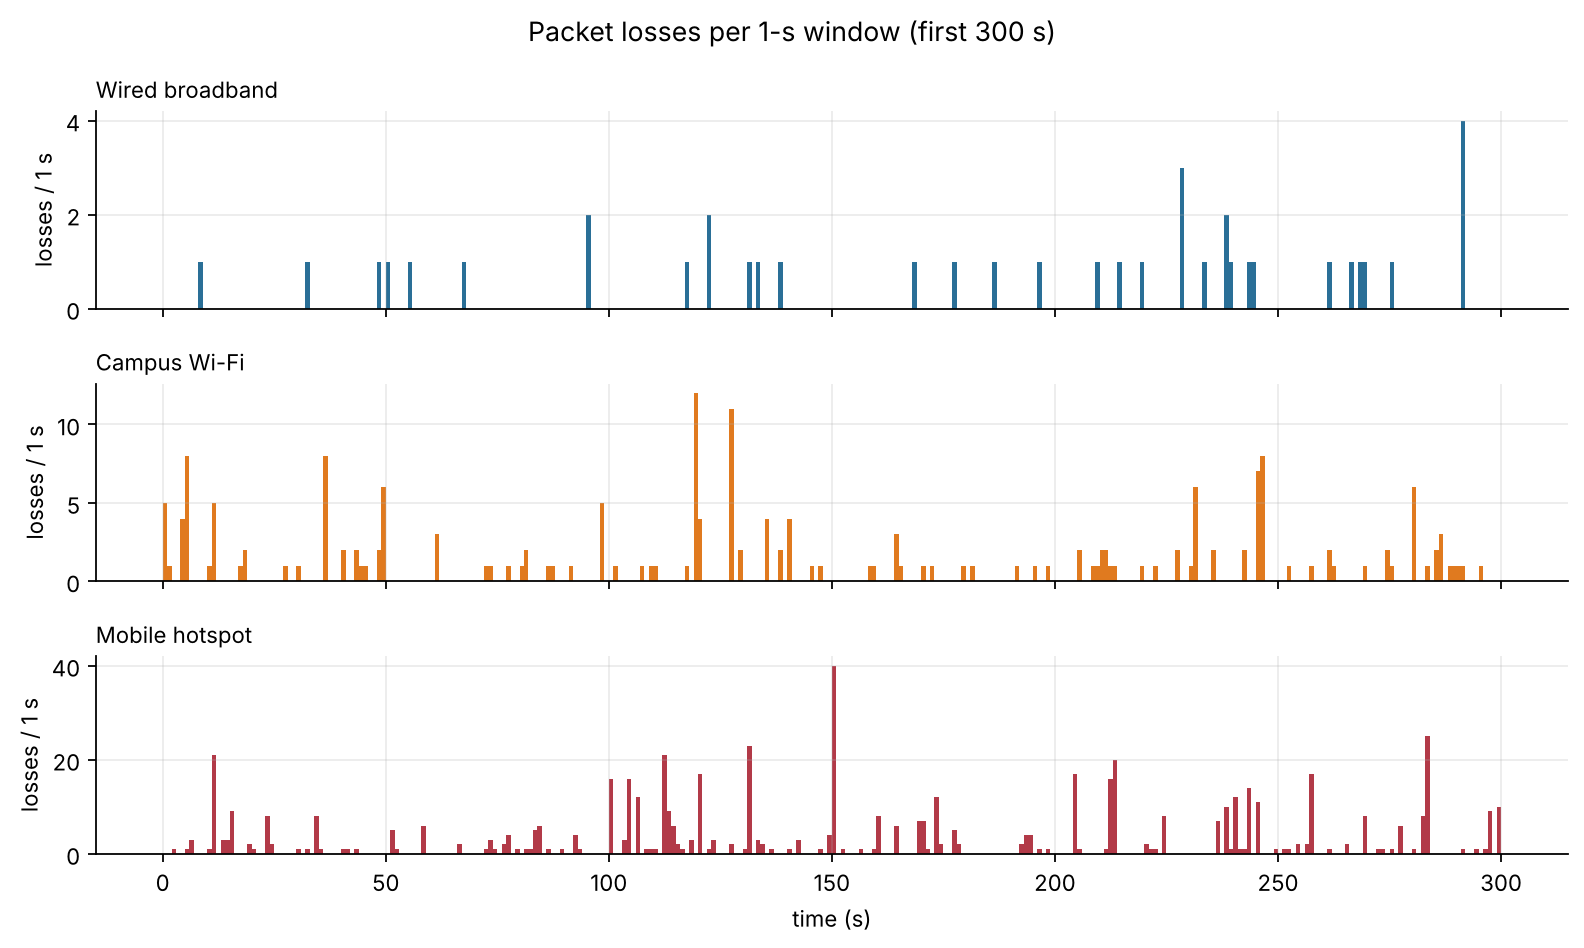
\includegraphics[width=\columnwidth]{fig1_loss_timeline.png}
\caption{Losses per second over the first five minutes of each simulated trace. On Wi-Fi and the mobile hotspot, losses arrive in clusters rather than one at a time.}
\label{fig:timeline}
\end{figure}

\section{Methodology}
\subsection{Fitting the Distributions}
For the loss counts per window, $x_1,\dots,x_n$, we start with the Poisson distribution. Its maximum-likelihood estimate is simply the average count, $\hat\lambda=\bar x$. The obvious alternative is the Negative Binomial:
\begin{align}
P(X=k)&=\binom{k+r_{\!NB}-1}{k}q^{r_{\!NB}}(1-q)^k,\\
\operatorname{Var}(X)&=\mu+\mu^2/r_{\!NB} .
\end{align}
One way to picture the Negative Binomial is as a Poisson whose rate keeps changing, which is exactly what happens when a network flips between good and bad periods. The extra term $\mu^2/r_{\!NB}$ lets the variance be bigger than the mean, which a Poisson cannot do. We fit it by keeping the mean at $\bar x$ and searching for the $r_{\!NB}$ that maximises the likelihood.

For the gaps between losses, the starting point is the exponential distribution, with $\hat\lambda=1/\bar t$. The alternative is a mixture of two exponentials, called a two-phase hyperexponential:
\begin{equation}
f(t)=w\lambda_1e^{-\lambda_1t}+(1-w)\lambda_2e^{-\lambda_2t}.
\end{equation}
The idea is that there are two kinds of gap. Short ones, with the fast rate $\lambda_1$, happen inside a burst. Long ones, with the slow rate $\lambda_2$, happen between bursts. We never know which kind a given gap is, so we fit the mixture with the Expectation-Maximisation (EM) algorithm. In each round, the E-step works out how likely each gap is to be a short one, and the M-step updates $w$, $\lambda_1$ and $\lambda_2$ using those probabilities as weights. We repeat until the fit stops improving. To compare models we use the Akaike Information Criterion, $\text{AIC}=2k-2\ln L$, which rewards a good fit but charges for every extra parameter. Lower is better.

\subsection{Goodness of Fit}
To check the count models, we compare the observed number of windows with each count against what the model expects, using the Pearson statistic $\chi^2=\sum_i (O_i-E_i)^2/E_i$. Small expected counts in the tail make this test unreliable, so we merge tail bins until every expected count is at least 5. The degrees of freedom are the number of bins, minus one, minus the number of fitted parameters. We also run the index-of-dispersion test. If the counts are Poisson, $(n-1)s^2/\bar x$ follows a $\chi^2_{n-1}$ distribution, so a variance much larger than the mean shows up as a very large statistic.

For the gaps, we use the Kolmogorov-Smirnov (KS) distance $D=\sup_t|F_n(t)-F(t)|$, the largest vertical gap between the data's cumulative curve and the model's. There is a catch here. The standard KS tables assume the model was fixed before looking at the data, but we estimate the rate from the same data, which flatters the fit and makes the textbook p-value too large. To get an honest p-value we use a parametric bootstrap. We simulate a fake data set from the fitted model, refit it, and record its $D$. Doing this 2{,}000 times for the exponential and 500 times for the mixture shows how large $D$ normally gets when the model really is correct.

\subsection{Testing Independence}
The Wald-Wolfowitz runs test looks at the 0/1 sequence of delivered and lost packets and counts the runs $R$, meaning stretches of identical outcomes. With $n_1$ losses and $n_0$ deliveries, independence predicts
\begin{equation}
E[R]=\frac{2n_1n_0}{n}+1,\quad \operatorname{Var}(R)=\frac{2n_1n_0(2n_1n_0-n)}{n^2(n-1)} .
\end{equation}
If losses stick together, there are fewer switches between lost and delivered than chance would give, so $R$ comes out too small.

The Markov-chain test asks a more direct question: does the fate of one packet depend on the packet before it? Under $H_0$ every packet has the same loss probability. Under $H_1$ there are two probabilities, $a=P(L\mid N)$ after a delivered packet and $b=P(L\mid L)$ after a lost one. If $n_{xy}$ is the number of times outcome $x$ is followed by outcome $y$,
\begin{equation}
\hat a=\frac{n_{NL}}{n_{NN}+n_{NL}},\qquad \hat b=\frac{n_{LL}}{n_{LN}+n_{LL}},
\end{equation}
\begin{equation}
G^2=2(\ln L_1-\ln L_0).
\end{equation}
Since $H_1$ has one more parameter than $H_0$, Wilks' theorem says $G^2$ is roughly $\chi^2_1$ when $H_0$ is true. The two estimates are also useful on their own. The ratio $b/a$ tells us how much one loss raises the chance of the next, and $1/(1-b)$ is the average burst length.

To compare the three networks we use rank-based tests, because the counts are mostly zeros, heavily skewed and nothing like normal. The Kruskal-Wallis test compares all three at once, and pairwise Mann-Whitney tests compare them two at a time, with a Bonferroni correction so that running three tests does not inflate the false-alarm rate. A $\chi^2$ test of homogeneity on the lost and delivered totals checks whether the loss proportion is the same everywhere. Every test uses $\alpha=0.05$.

\subsection{Bayesian Estimation}
For the loss rate itself, we take a Bayesian view. We start from a flat $\text{Beta}(1,1)$ prior, which says every loss rate between 0 and 1 is equally plausible before we see any data. After seeing $k$ losses in $n$ packets, the posterior is $\text{Beta}(1+k,\,1+n-k)$. In other words, we simply add the losses and deliveries to the prior counts. We report the posterior mean and the 95\% credible interval, and we show for Campus Wi-Fi how the posterior narrows as more traffic comes in. To check whether the networks really are ordered by loss rate, we draw 200{,}000 values from each posterior and count how often Wired $<$ Wi-Fi $<$ Mobile.

The same idea works for the burst parameters. We give $a$ and $b$ their own posteriors, $a\sim\text{Beta}(1+n_{NL},1+n_{NN})$ and $b\sim\text{Beta}(1+n_{LL},1+n_{LN})$, and from them get credible intervals for $b/a$ and the burst length. As a sanity check on the independent model, we also ask it to predict how often a window should contain at least 5 losses, and compare that with how often it actually does.

\subsection{Design Effect}
The reason bursts cause trouble for interval estimates shows up in the variance of a sum:
\begin{equation}
\operatorname{Var}\Big(\sum_i X_i\Big)=\sum_i\operatorname{Var}(X_i)+2\sum_{i<j}\operatorname{Cov}(X_i,X_j).
\end{equation}
If packets were independent, the covariance terms would all be zero and the variance of the loss count would be $np(1-p)$. Inside a burst, neighbouring packets tend to share the same fate, so the covariances are positive and the real variance is larger. The standard interval ignores this and comes out too narrow.

To correct for it, we split each trace into blocks of $m=500$ packets (10~s) and compare the real spread of the block counts with what independence would give:
\begin{equation}
\text{deff}=\frac{s^2_{\text{block}}}{m\,\hat p(1-\hat p)},\qquad n_{\text{eff}}=\frac{n}{\text{deff}},
\end{equation}
with deff never allowed below 1. You can read $n_{\text{eff}}$ as the number of independent packets that our correlated packets are worth. The adjusted posterior uses these effective counts, $\text{Beta}(1+k/\text{deff},\,1+(n-k)/\text{deff})$, which gives a wider and more honest interval.

\subsection{Monte Carlo Checks}
Two questions cannot be answered from a single trace, so we answer them by repeating the experiment many times. The first is power: how likely is each test to notice the bursts? For capture lengths from 15~s to 600~s, we simulate 2{,}000 captures per network and count how often each test rejects independence. The second is coverage: how often does a 95\% interval actually contain the true loss rate? We simulate 2{,}000 captures of 10 minutes per network, build the naive and the adjusted interval for each, and count the hits. With 2{,}000 repeats, each of these proportions is accurate to within about 0.011 (one standard error).

\section{Results}
\begin{figure*}[!tb]
\centering
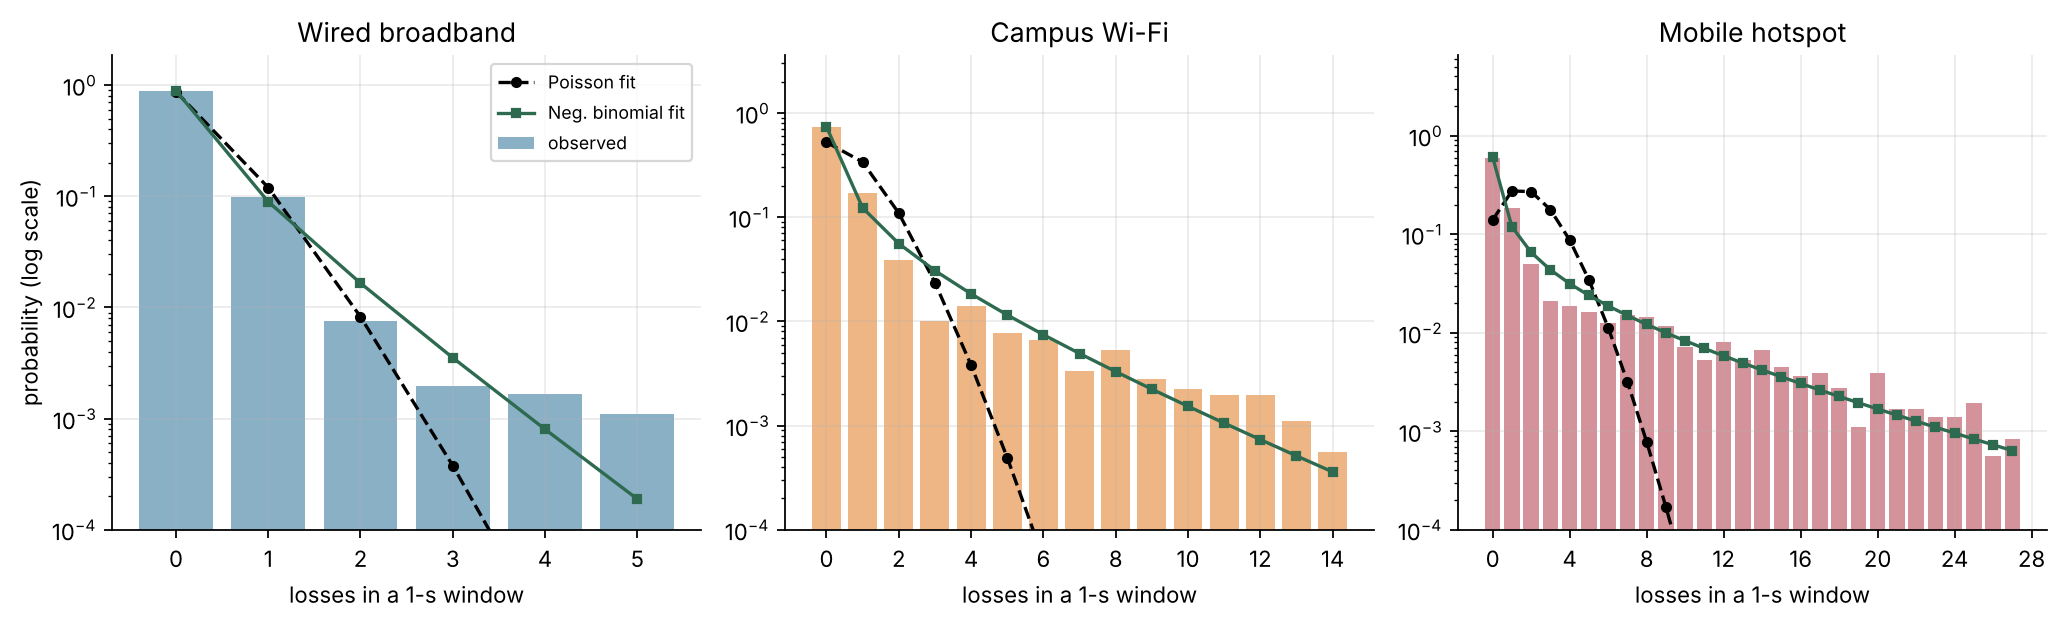
\includegraphics[width=0.92\textwidth]{fig2_count_distribution_fits.png}
\caption{Probability of $k$ losses in one second, on a log scale. The Poisson fit (dashed) drops far below the real tail; the Negative Binomial (green) follows it.}
\label{fig:counts}
\end{figure*}

\subsection{Loss Counts}
The Poisson model fails on all three networks. Table~\ref{tab:counts} shows why. For a Poisson distribution the variance should equal the mean, but here it is 1.59, 5.31, 10.17 times the mean, and the dispersion test gives $p<10^{-10}$ every time. The Negative Binomial fits much better and has a lower AIC on every network. The biggest improvement is on Mobile, where the AIC drops from 25{,}042 to 11{,}700.

Most of the difference sits in the tail. On Wi-Fi, the Poisson model expects about 1.98 seconds with 5 or more losses in an hour. The trace actually has 131. The Negative Binomial expects 124.2, which is close. Fig.~\ref{fig:counts} shows this on a log scale: the Poisson curve falls away almost immediately, while the real counts and the Negative Binomial carry on.

\begin{figure*}[!tb]
\centering
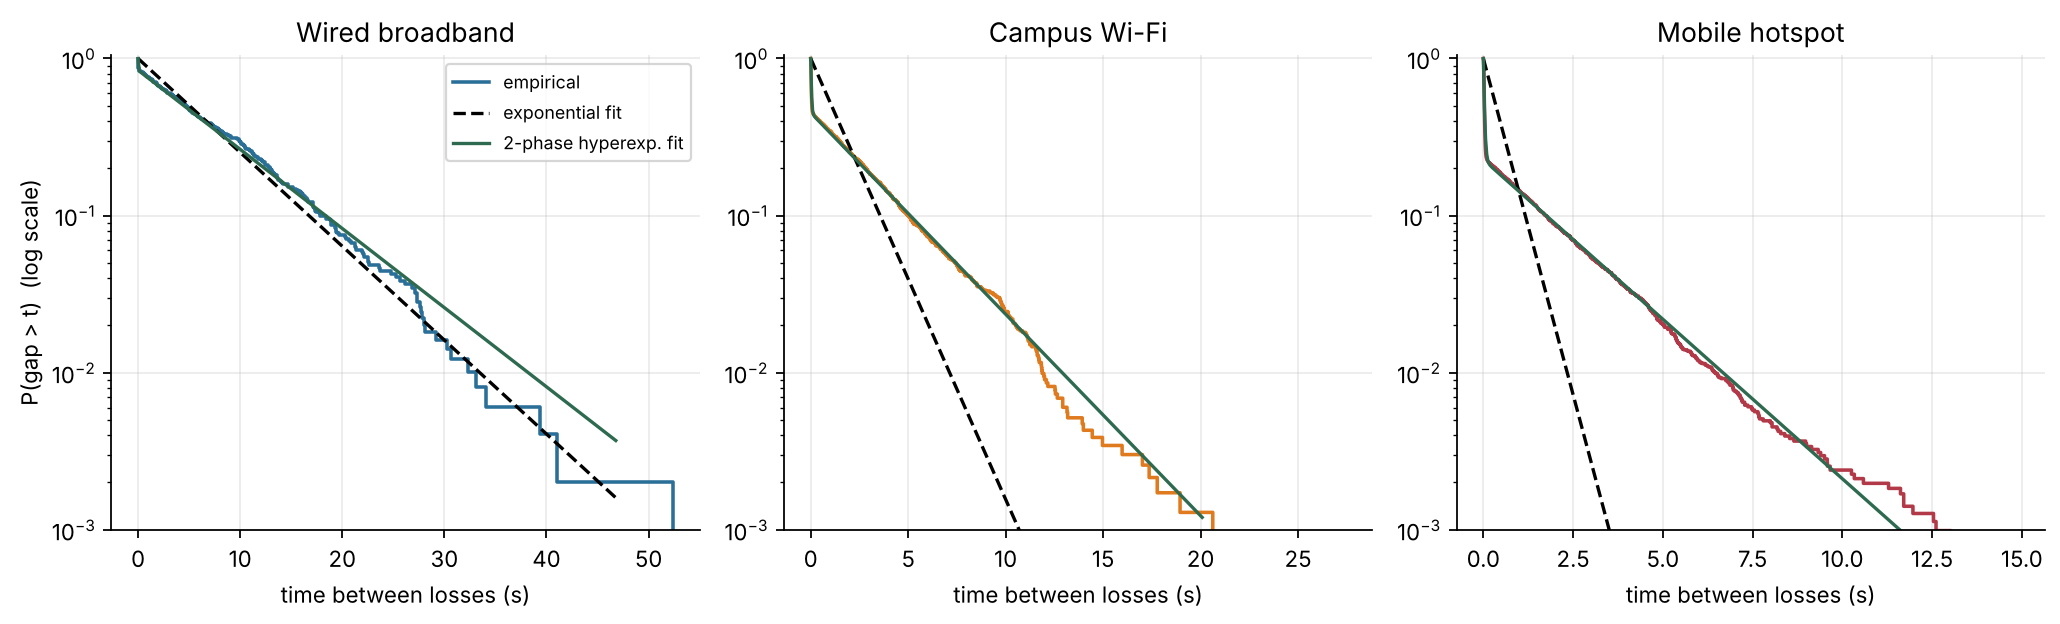
\includegraphics[width=0.92\textwidth]{fig3_gap_survival.png}
\caption{Probability that a gap between losses is longer than $t$, on a log scale. An exponential gives a straight line (dashed); the two-phase mixture (green) bends with the data.}
\label{fig:gaps}
\end{figure*}

\begin{table*}[!tb]
\caption{Losses per second and how well the count models fit}
\label{tab:counts}
\centering
\footnotesize
\setlength{\tabcolsep}{6pt}
\begin{tabular}{lcccccccc}
\toprule
Network & Loss rate & Mean / s & Variance & D & $\chi^2$ Poisson & AIC Poisson & AIC Neg. Bin. & Seconds with $\ge$5 losses \\
\midrule
Wired & 0.275\% & 0.138 & 0.219 & 1.59 & 22.5 & 3{,}143 & 2{,}992 & 7 / 0.00132 / 0.9 \\
Wi-Fi & 1.292\% & 0.646 & 3.430 & 5.31 & 2{,}544.2 & 10{,}607 & 7{,}186 & 131 / 1.98 / 124.2 \\
Mobile & 3.937\% & 1.969 & 20.017 & 10.17 & 15{,}840.8 & 25{,}042 & 11{,}700 & 487 / 180 / 492.0 \\
\bottomrule
\end{tabular}
\\[2pt]
\raggedright\scriptsize D is the variance divided by the mean. The last column gives the number of seconds with at least 5 losses: observed / expected under Poisson / expected under Negative Binomial. Every Poisson test gives $p<10^{-10}$.
\end{table*}

\FloatBarrier
\subsection{Gaps Between Losses}
The exponential model fails too. The bootstrap KS test rejects it on every network (Table~\ref{tab:gaps}). The easiest way to see the problem is Fig.~\ref{fig:gaps}. On a log scale, an exponential survival curve is a straight line. The real curves are not. They drop steeply at the start, because many gaps are tiny, and then flatten out, because the rest are long.

The two-phase mixture captures this shape well. Its fast phase has an average gap of 29 to 33~ms, which is one or two packets, so these are the gaps inside a burst. Its slow phase averages 2.1 to 8.6~s, which is the quiet time between bursts. The share of gaps in the fast phase grows from 16\% on Wired to 77\% on Mobile, which fits the idea that the mobile link spends more of its losses in bursts. The mixture passes the KS test on Wired ($p=0.154$) and cuts the AIC sharply on all three networks. It is still rejected on Wi-Fi and Mobile, though, so it is a big improvement rather than a perfect description.

\begin{table}[!htbp]
\caption{Gaps between losses: exponential and two-phase fits}
\label{tab:gaps}
\centering
\footnotesize
\setlength{\tabcolsep}{3pt}
\begin{tabular}{lccccccc}
\toprule
Net. & $w$ & Fast & Slow & \multicolumn{2}{c}{KS $p$} & \multicolumn{2}{c}{AIC} \\
 & & (ms) & (s) & exp. & mix. & exp. & mix. \\
\midrule
Wired & 16\% & 32 & 8.6 & $<0.0005$ & 0.154 & 2{,}950 & 2{,}644 \\
Wi-Fi & 55\% & 33 & 3.4 & $<0.0005$ & $<0.002$ & 6{,}682 & 1{,}368 \\
Mobile & 77\% & 29 & 2.1 & $<0.0005$ & $<0.002$ & 4{,}563 & -15{,}477 \\
\bottomrule
\end{tabular}
\\[2pt]
\raggedright\scriptsize $w$ is the share of gaps in the fast phase. Fast and slow are the average gap in each phase.
\end{table}

\FloatBarrier
\subsection{Do Losses Depend on Each Other?}
Yes, strongly. Both independence tests reject $H_0$ with $p<10^{-10}$ on every network (Table~\ref{tab:dep}). On Wi-Fi we count 3{,}005 runs where independence would give about 4{,}593, a $z$-score of -146.7. The Markov estimates make the effect easy to picture. On Wi-Fi, a packet that follows a delivered packet is lost 0.85\% of the time. A packet that follows a lost packet is lost 35.4\% of the time.

The posterior medians of $b/a$ are 43, 42, 31 for Wired, Wi-Fi and Mobile, so one loss makes the next 31 to 43 times more likely (Fig.~\ref{fig:markov}). The posterior probability that $b>a$ is 1.000 on every network, so there is no real doubt about the direction of the effect. Average bursts are short, 1.12, 1.55, 2.25 packets, but they are much more common than chance would allow.

\begin{figure}[!htbp]
\centering
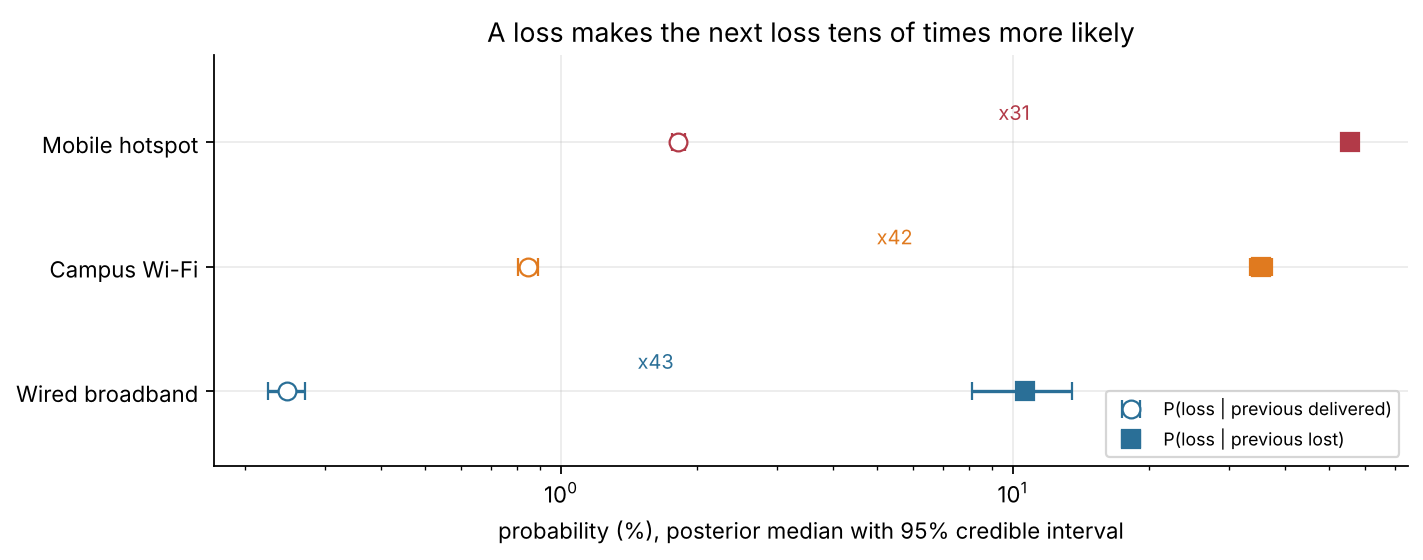
\includegraphics[width=\columnwidth]{fig5_markov_posteriors.png}
\caption{Posterior medians and 95\% credible intervals for $P(L\mid N)$ (open) and $P(L\mid L)$ (filled). On every network a loss makes the next loss far more likely.}
\label{fig:markov}
\end{figure}

\begin{table}[!htbp]
\caption{Tests of independence and burst parameters}
\label{tab:dep}
\centering
\footnotesize
\setlength{\tabcolsep}{2.2pt}
\begin{tabular}{lcccccccc}
\toprule
Net. & Runs & $E[R]$ & $z$ & $G^2$ & $P(L|N)$ & $P(L|L)$ & $b/a$ & Burst \\
\midrule
Wired & 887 & 988 & -43.5 & 288.4 & 0.25\% & 10.5\% & 43 & 1.12 \\
Wi-Fi & 3{,}005 & 4{,}593 & -146.7 & 4{,}498.6 & 0.85\% & 35.4\% & 42 & 1.55 \\
Mobile & 6{,}293 & 13{,}617 & -228.2 & 18{,}560.2 & 1.82\% & 55.6\% & 31 & 2.25 \\
\bottomrule
\end{tabular}
\\[2pt]
\raggedright\scriptsize $b/a$ and burst length (in packets) are posterior medians. All $p<10^{-10}$.
\end{table}

\begin{figure*}[!tb]
\centering
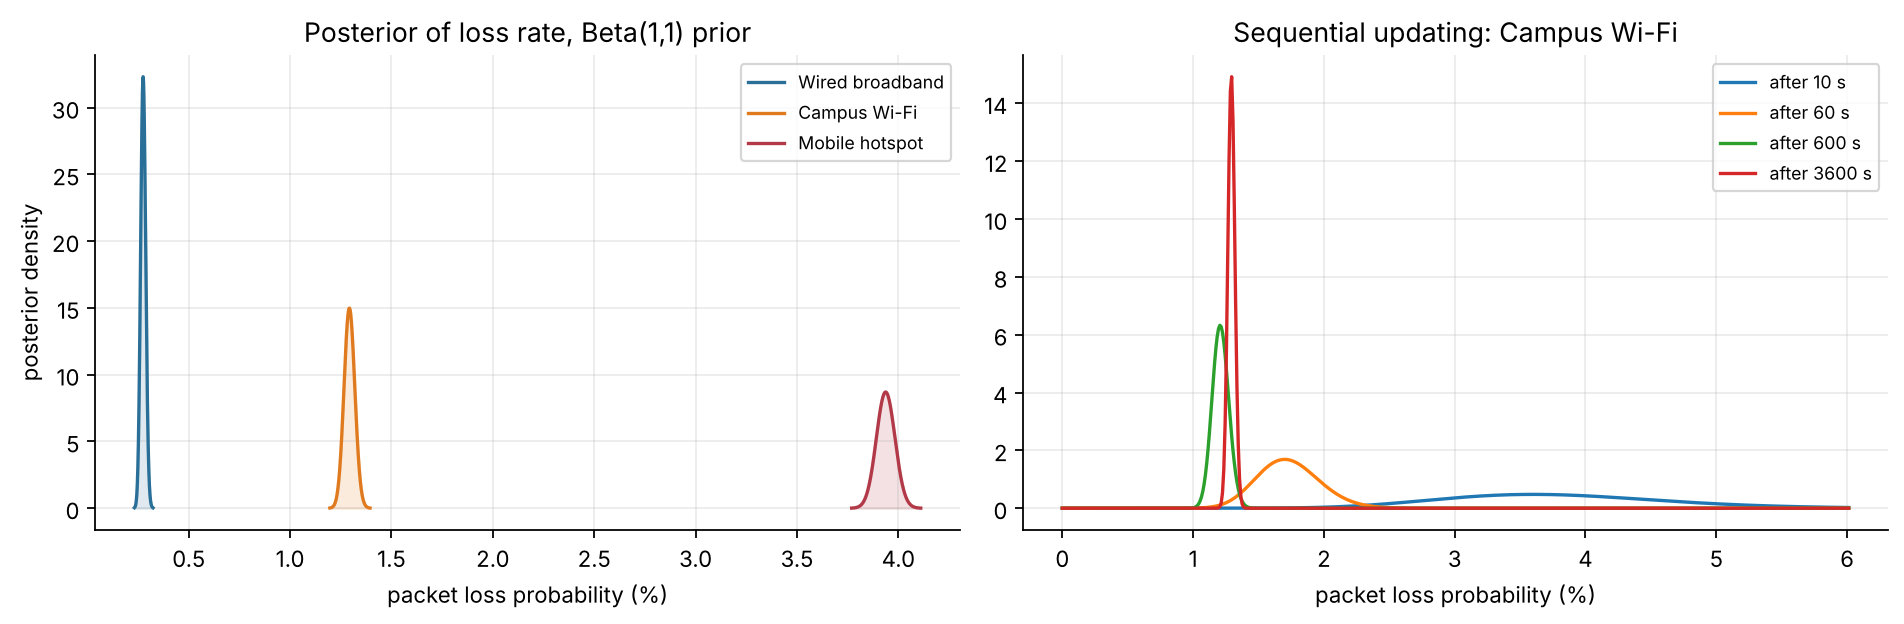
\includegraphics[width=0.92\textwidth]{fig4_bayesian_posteriors.png}
\caption{Left: posterior distributions of the loss rate for the three networks. Right: the Wi-Fi posterior after 10~s, 60~s, 600~s and 3,600~s of traffic.}
\label{fig:bayes}
\end{figure*}

\FloatBarrier
\subsection{Comparing the Networks}
As expected from how we set them up, the three networks are clearly different. The Kruskal-Wallis statistic is $H=937.3$, the $\chi^2$ homogeneity statistic is 7{,}143.0 on 2 degrees of freedom, and even the largest Bonferroni-corrected pairwise p-value is $<10^{-10}$. The posterior mean loss rates are 0.276\%, 1.293\%, 3.938\% (Table~\ref{tab:bayes}), and the posterior probability of the order Wired $<$ Wi-Fi $<$ Mobile is 1.000.

Fig.~\ref{fig:bayes} shows the Bayesian side of this. After only 10~s of Campus Wi-Fi traffic, the estimate is 3.78\% [2.30\%, 5.62\%], which is wide. After 3{,}600~s it has tightened to 1.29\% [1.24\%, 1.35\%].

The predictive check shows how badly the independent model handles heavy seconds. On Wi-Fi it says a second with at least 5 losses should happen with probability 0.00047. In the trace, it happens 0.036 of the time, roughly 77 times more often.



\FloatBarrier
\subsection{How Often Do the Intervals Work?}
This is the result we think matters most. Over 2{,}000 simulated 10-minute captures, the naive 95\% interval contained the true loss rate in only 85.7\%, 60.9\%, 40.3\% of cases (Table~\ref{tab:bayes}, Fig.~\ref{fig:coverage}). On the burstiest network it was wrong more often than it was right.

\begin{figure}[!htbp]
\centering
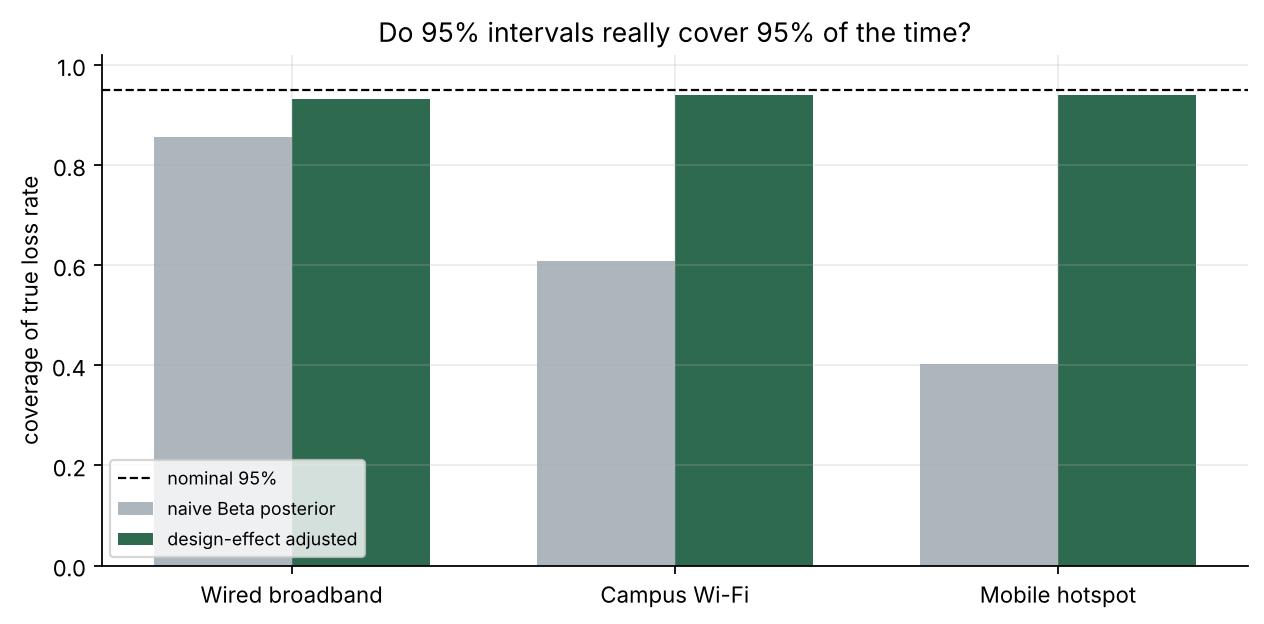
\includegraphics[width=\columnwidth]{fig7_interval_coverage.png}
\caption{How often the nominal 95\% interval contains the true loss rate, before and after the design-effect correction.}
\label{fig:coverage}
\end{figure}

\begin{figure*}[!tb]
\centering
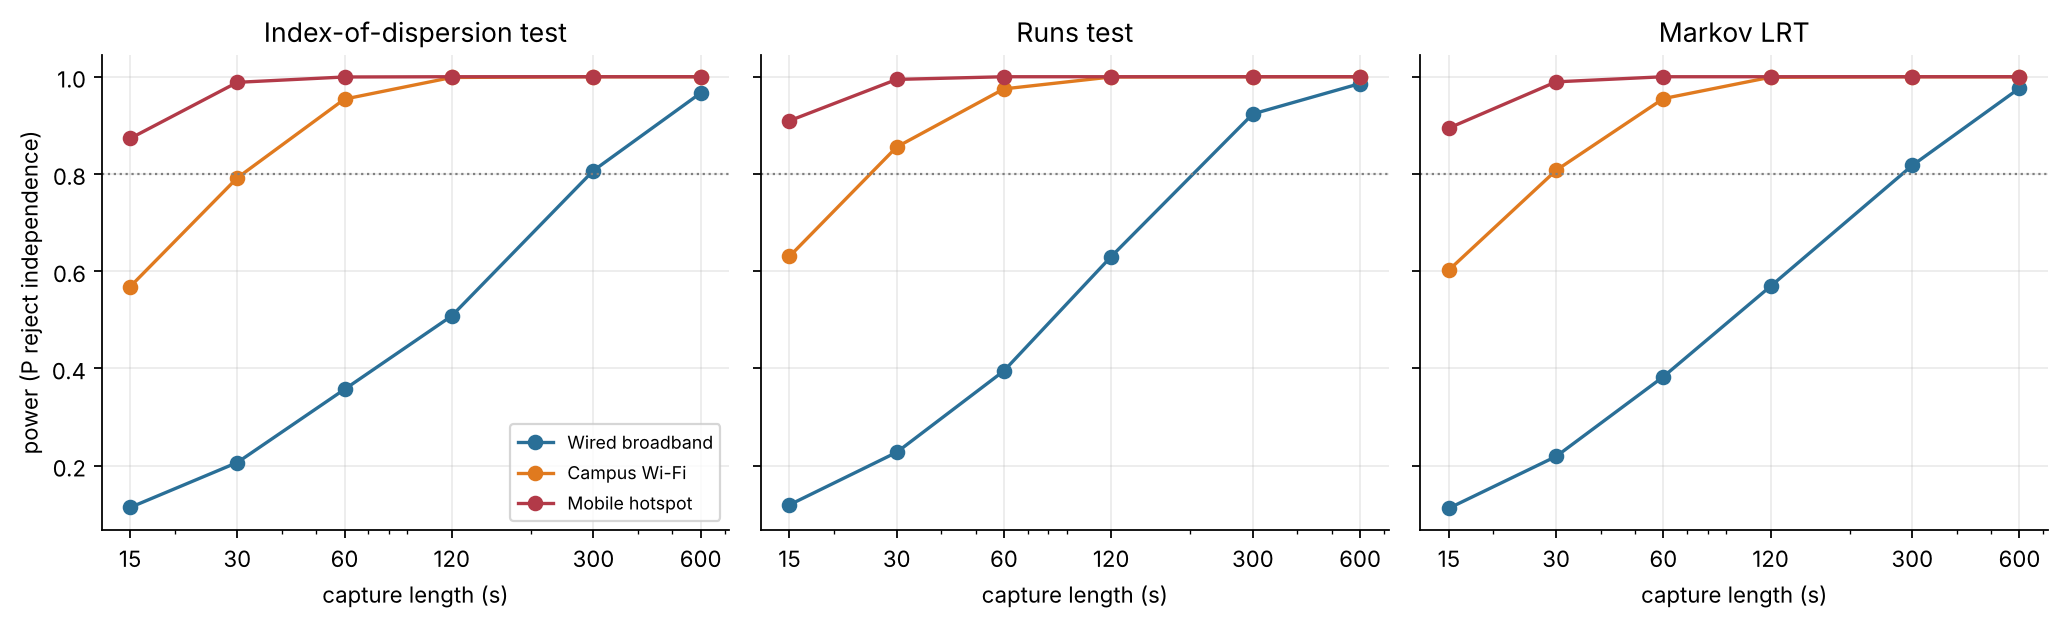
\includegraphics[width=0.92\textwidth]{fig6_power_curves.png}
\caption{Power to detect dependence against capture length, from 2{,}000 simulated captures per point. The dotted line marks a power of 0.8.}
\label{fig:power}
\end{figure*}

The design effects are 1.52, 6.43 and 12.14. On Wi-Fi, that means our 180{,}000 packets carry about as much information as 28{,}000 independent ones. Once we use these smaller effective sample sizes, coverage comes back to 93.3\%, 94.0\%, 94.0\%, close to the 95\% it should be. The price is a wider interval. On Wi-Fi the average width grows from 0.245 to 0.563 percentage points, but a wider interval that is right is more useful than a narrow one that is wrong.

The full Wi-Fi trace gives a concrete example. The true loss rate is 1.184\%. The naive interval, [1.241\%, 1.345\%], misses it completely. The adjusted interval, [1.167\%, 1.431\%], contains it.

\begin{table*}[!tb]
\caption{Loss-rate estimates and coverage of 95\% intervals}
\label{tab:bayes}
\centering
\footnotesize
\setlength{\tabcolsep}{8pt}
\begin{tabular}{lcccccc}
\toprule
Network & Posterior mean & Naive 95\% interval & deff & Adjusted 95\% interval & Naive coverage & Adjusted coverage \\
\midrule
Wired & 0.276\% & [0.252\%, 0.300\%] & 1.52 & [0.247\%, 0.307\%] & 85.7\% & 93.3\% \\
Wi-Fi & 1.293\% & [1.241\%, 1.345\%] & 6.43 & [1.167\%, 1.431\%] & 60.9\% & 94.0\% \\
Mobile & 3.938\% & [3.848\%, 4.028\%] & 12.14 & [3.636\%, 4.263\%] & 40.3\% & 94.0\% \\
\bottomrule
\end{tabular}
\\[2pt]
\raggedright\scriptsize Intervals are from the full 1-hour trace. Coverage is from 2{,}000 simulated 10-minute captures.
\end{table*}



\FloatBarrier
\subsection{How Long Should a Capture Be?}
Fig.~\ref{fig:power} shows how the power of each test grows with the length of the capture, and Table~\ref{tab:power} gives the shortest length we tried that reaches a power of 0.8. With the runs test, the mobile network needs only 15~s and Wi-Fi 30~s. Wired needs 300~s, because its bursts are rare and short, so it takes longer to collect enough evidence. The runs test was the most powerful of the three on every network. At 600~s, every test has a power of at least 0.97 on every network, so we plan to record at least ten minutes per network in Phase 2.

\begin{table}[!htbp]
\caption{Shortest capture (s) with power of at least 0.8}
\label{tab:power}
\centering
\footnotesize
\begin{tabular}{lcccc}
\toprule
Network & Dispersion & Runs & Markov & Min. power at 600 s \\
\midrule
Wired & 300 & 300 & 300 & 0.97 \\
Wi-Fi & 60 & 30 & 30 & 1.00 \\
Mobile & 15 & 15 & 15 & 1.00 \\
\bottomrule
\end{tabular}
\end{table}



\section{Discussion and Limitations}
The striking thing is how little it takes. A Bad spell lasting just a few packets is enough to break every model that assumes independence. The loss rate on its own hides this completely. Mobile loses about 14 times as many packets as Wired, yet on both of them a loss makes the next loss tens of times more likely. Burstiness is a separate property of a link, and it has to be measured separately.

The coverage results show why this matters beyond modelling. A naive interval treats every packet as a fresh piece of evidence. When packets inside a burst share the same fate, there is much less independent evidence than the packet count suggests, and the interval ends up too narrow. The effect gets worse as the network gets burstier, which is why Mobile has the lowest naive coverage. The design-effect fix is simple, needs nothing more than block counts, and brings coverage close to 95\% on all three networks.

There are several limits to what we can claim. The biggest is that the data are simulated, and from the same kind of model that motivated the study. The tests themselves do not use this knowledge, and we only use the true parameters to judge the estimates, but real links have other effects, such as busy hours, that our model leaves out. Phase 2 is meant to address this.

Some smaller points are worth stating too. The dispersion test compares the counts against a Poisson, while counts out of 50 packets are really Binomial, with a variance slightly below the mean. This makes the test a little cautious, so if anything it understates burstiness. The runs and Markov tests rely on large-sample approximations. In very short captures their false-alarm rate can drift away from 5\%, although it stays close to 5\% for hour-long traces. The Negative Binomial and the two-phase mixture are still rejected on Wi-Fi and Mobile, so neither is the full story. The design effect depends on the block length; our 10-s blocks are much longer than any Bad spell, which should be enough. Finally, the headline numbers come from one seeded trace per network, although the Monte Carlo checks repeat the whole experiment thousands of times.

\section{Conclusion and Future Work}
We tested whether packet losses behave independently on three simulated networks, and they do not. The Poisson and exponential models were rejected everywhere. Losses per second were 1.59, 5.31, 10.17 times more spread out than Poisson allows, the gaps split into short in-burst gaps and long quiet gaps, and a loss made the next one 31 to 43 times more likely. Most importantly, the usual 95\% interval for the loss rate was right only 40.3\% to 85.7\% of the time, and dividing the sample size by the design effect raised this to 93.3\% to 94.0\%.

The next step is Phase 2. We will record steady 50-packets-per-second streams on real wired, Wi-Fi and mobile links, for at least ten minutes each, and run the same code on them. After that, we would like to estimate the Gilbert-Elliott parameters directly from the real traces with the Baum-Welch algorithm, try richer models for the tail, use the Phase 1 results as priors in a hierarchical Bayesian model across networks, and compare loss at peak and off-peak hours.

\section*{Reproducibility}
All results come from a single Python pipeline built on NumPy, SciPy and Matplotlib, run with seed 2026. Rerunning it regenerates every table and figure in this report.

\end{document}
